\chapter{Evaluation\label{chap:evaluation}}
  This chapter will detail the evaluation metrics, how they were used to test the performance of the tool and what the results of the evaluation were. Two studies were carried out making use of six debates from our corpus \cite{walker2012corpus}: abortion, creation, gay rights, the existence of god, gun ownership and healthcare. A final study was carried out making use of the same debate summaries and two new summaries for discussion on Twitter around the 2014 Independence Referendum.

  \section{Research Questions}
    We wanted to evaluate our tool as an automatic summarization tool. The result of a final analysis stage was a summary comprising of point extracts for a given debate, by assessing the quality of this we can also evaluate the precursor points extraction analysis. The following research questions were set:

    \begin{itemize}
      \item{Are our summaries more readable and informative than those produced by existing tools?}
      \item{Does introducing summary sections with an explanation improve readability?}
      \item{How well does our bigram-based extract selection perform?}
      \item{Which sections of generated summaries are most and least useful to readers?}
    \end{itemize}

    To address these questions we compared different versions of our summaries against equal-length summaries generated by an implementation \footnote{http://homepages.abdn.ac.uk/advaith/pages/teaching/NLP/practicals/Practical3.zip} of the approach described by Nenkova et al. \cite{nenkova2006compositional}. We also gathered scores for groups of extracts allocated by the bigram model for comparison with human scores. Additionally, summaries generated with randomly selected extracts against were compared against one based on our bigram model for selection.

  \section{Design}
    In response to the our research questions we set the following null hypotheses for the evaluation:

    \begin{itemize}
      \item{The readability and informativeness of our summaries do not improve on those of existing tools. (\textbf{H1})}
      \item{Explanations introducing summary sections does not improve readability. (\textbf{H2})}
      \item{Our means of selecting extracts is not better than random selection. (\textbf{H3})}
      \item{All summary sections are equally useful to readers. (\textbf{H4})}
    \end{itemize}

    \tocless\subsection{Study Participants}
      To test these hypotheses, we prepared three comparative studies. These are described in Sections \ref{sec:stud1} onwards. Participants for studies 1 and 2 were recruited using Amazon Mechanical Turk. In the both studies, workers were required to be `Mechanical Turk Masters', these workers have \blockquote{\textit{demonstrated excellence across a wide range of [Human Intelligence Tasks]}}. Study 1, comparing summaries, had 26 unique participants giving 55 responses to 6 different tasks. Study 2, rating extracts, had 27 unique participants giving 55 responses to 6 different tasks. There were 38 participants in total across both studies, each participant could not complete the same task more than once. The average worker had completed 3 tasks and had an approval rating of 98\%.

      For Study 3 we attended a workshop with social science researchers interested in using social media analysis in their work. There were 15 present and we collected written comments from 9.

    \tocless\subsection{Summary Styles}
      In the upcoming sections, reference is made to a range of summary styles used in evaluation tasks.
      \begin{itemize}
        \item{\textbf{Stock}: A summary generated using an implementation of the approach described by Nenkova et al. \cite{nenkova2006compositional}. These stock summaries were used as a benchmark for summaries generated by our tool. There is no structure to these summaries, they are generated by selecting sentences that reference prominent words not already included in the summary. The resulting distribution of words in the summary is close to that of the input text.}
        \item{\textbf{Plain}: This is a collection of point extracts in the same style as the stock summaries. The extracts are still grouped into sections, only this is not made clear in the presentation. Plain summaries were designed to be as close as possible to the stock summary presentation. Plain summaries were also of equal length to the benchmark stock summaries.}
        \item{\textbf{Layout}: A summary that has explanatory text that introduces sections. The extracts are the same as those in the plain summary though the explanations increase the overall word count. For a fair evaluation, these are compared against a longer stock summary..}
        \item{\textbf{Formatted}: A layout summary with explanation keywords in bold and topic words in green. The content is the same as a layout summary.}
      \end{itemize}

    \tocless\subsection{Study 1: Summary Comparison\label{sec:stud1}}
      In order to address \textbf{H1} and \textbf{H2} we designed a questionnaire that compared various summary styles against equal-length stock summaries. Each questionnaire was made up of three sections. Please see Appendix \ref{app:survey-section} for an example summary section.

      The first section compared a plain summary against a stock summary on the same topic. Users were instructed to read both summaries and rate them relatively on the following criteria:

      \begin{itemize}
        \item{Content Interest / Informativeness}
        \item{Readability}
        \item{Punctuation \& Presentation}
        \item{Organization}
      \end{itemize}

      Finally they were asked to give an overall rating and justify their response using free text. The following section asked the same questions but instead compared a layout summary against a stock one - this second comparison was for a different topic. Layout summaries are longer because of the explanatory text, the stock summary was the same length as the layout summary and was longer than the stock summary used in the first section. The final section compared a layout summary with a formatted one. The layout summary is reused from the second section, the formatted summary has the same content (only different formatting). There was only an overall rating and justification for the comparison in this section.

      There were six versions of the questionnaire setup in a Latin square to cover all six topics. Section 1 had a different topic from sections 2 so as to not repeat summary content. Section 3 addresses the question of formatting only and has the same content as the layout summary in section 2 to make the task faster.

      Responses from the first section that compare our plain summary against a stock one can be used in addressing \textbf{H1}. The difference in the responses gathered in section 2 will allow us to address \textbf{H2}. Section 3 expands on this, testing if the formatting is a useful addition to the layout summary.

    \tocless\subsection{Study 2: Extract Comparison}
    To investigate the performance of the tool in greater depth we ran a further study testing the quality of our extract selection mechanism. Responses from this questionnaire addressed \textbf{H3}. See Appendix \ref{app:extract-survey-section} for an example section.

    The task given to participants had two sections. First were three sets of extracts for three different point patterns, participants were asked to rate extracts accounting for their succinctness and the extent to which they made sense. This was the closest we could make the task for participants to that of the aim of the tool. The following section, similar to the first study, compared two summaries (see Appendix \ref{app:survey-comparison}). Both summaries were of the formatted style however this time their content differed. The extracts in one summary were selected using the bigram model, the extracts in the other were selected at random from the same clusters of points. Participants were asked to give these a relative rating and justify their response. Responses for these two tasks were intended to address \textbf{H3}.

    \tocless\subsection{Study 3: Section Comparison}
      This study was completed as a paper exercise with workshop participants in a session before the approach was discussed. Participants were given side-by-side summary comparisons, similar to the first study, however only qualitative feedback was requested. Given two comparisons of layout and stock summaries on two different topics, participants were prompted to:

      \blockquote{
        \textit{
          Write your comments about the two summaries. Feel free to
          say anything that strikes you, but particularly address:
          \begin{itemize}
            \item{Which you prefer, and why?}
            \item{Do you like the structuring into sections in one of the summaries?}
          \item{Which sections are most interesting to you?}
          \item{What other sections might be useful to you that are missing?}
          \end{itemize}
        }
      }

      Responses from this task were intended to answer to \textbf{H4}. We also introduced two new summaries: `Before Referendum' \& `Referendum Day' based on tweets referencing the \#indyref tag or mentioning one of the campaign accounts for those date ranges. One of these summaries made up the second comparison for each participant. The first comparison was selected from either: \textit{Abortion}, \textit{Gay Rights}, \textit{Existence of God} or \textit{Gun Laws}. These four were selected from the six available as they had all summary sections complete.

  \section{Results}
    \tocless\subsection{Study 1: Summary Comparison}
      The results of the summary comparison showed a strong preference for summaries based on points based extraction. When comparing the plain and stock summaries, our plain summaries were marked as better or much better by 69\% of participants. Plain summaries, lacking any kind of layout, were still scored better on organization by 57\% of participants.

      When comparing layout summaries against equal length stock summaries participant preference only became clearer. 89\% of participants rated the layout summary as better or much better than stock. Organization saw the greatest change, with a 30\% increase in favor of layout summaries.

      There was also variation between summaries of different discussions. The gay rights layout summary saw an increase of 45\% in better/much better scores while the guns layout summary saw no improvement. When comparing plain and stock summaries on guns and healthcare all participants rated plain as being the same or better. When comparing the healthcare layout and stock summaries all participants marked the layout summary as being much more readable. The plain vs. stock creation summary was the most divided, 42\% of responses were marked as same or stock better.

      Despite the point content used in the layout and plain summaries being the same, the `Content' factor saw an increase of 14\% in better/much better scores. Punctuation was also saw a 13\% increase, despite also being the same across both plain and layout summaries.

      Regarding the results of the layout / formatted summary comparison, more than half of respondents preferred the formatted version of the summary. This is considerably lower than the improvements of layout vs. stock (89\%) or even plain vs. stock (69\%).

      These findings are based on the 55 responses from 6 different questionnaires giving 165 summary comparisons. The target population was people interested in online discussions.

      To test the significance of these results we use one-sided Sign test for matched pairs. Neutral responses were excluded, better \& much better responses were amalgamated. When comparing plain against stock, 38 successes in 45 trials, we found the probability for success is not equal with $p << 0.01$ (\textbf{H1}). Comparing layout and stock summaries, 49/53, we found that success is also not equal, $p << 0.01$. However, when comparing the layout and formatted summaries, 29/41, we found $p = 0.16$ and thus unsuitable to reject the null hypothesis at this level. These results are based on all responses across all 6 debate topics.

      (need to show that the layout improves on the plain vs. stock, not sure how adjust my data to a Friedman Rank Sum Test)

      To conclude, the results show a preference for points based summaries. This can further be improved by introducing sections (if I can show statistical significance?). However we cannot say decisively that our formatted summaries improve on our layout versions.

    \tocless\subsection{Study 2: Extract Comparison}
      Extracts selected by our tool for display were scored above the user's mean score 74\% of the time. Selected extracts scored 3.94/5 on average while extracts not selected scored 3.11/5.

      (Results of a Mann-Whitney U test, or some other means of comparing the selected vs. not extracts regarding the values from the likert scale scores. This is quite hard\dots)

      Currently results of a MWU test would read (where A is selected and B is not selected by the tool): The medians of Group A and Group B were 5 and 3, respectively. We ran a Mann-Whitney's U test to evaluate the difference in the responses of our 5-Likert scale question. We found a significant effect of Group (The mean ranks of Group A and Group B were 1026 and 767, respectively; U = *155681*, Z = *7.045*, p= 1.851 * 10\^-12, r = 0.0.17).

      \begin{figure}[h]
        \caption{\textcolor{red}{SAMPLE PLOT, machine z scores vs. z scores of \textit{mean} human ratings}}
        \centering
        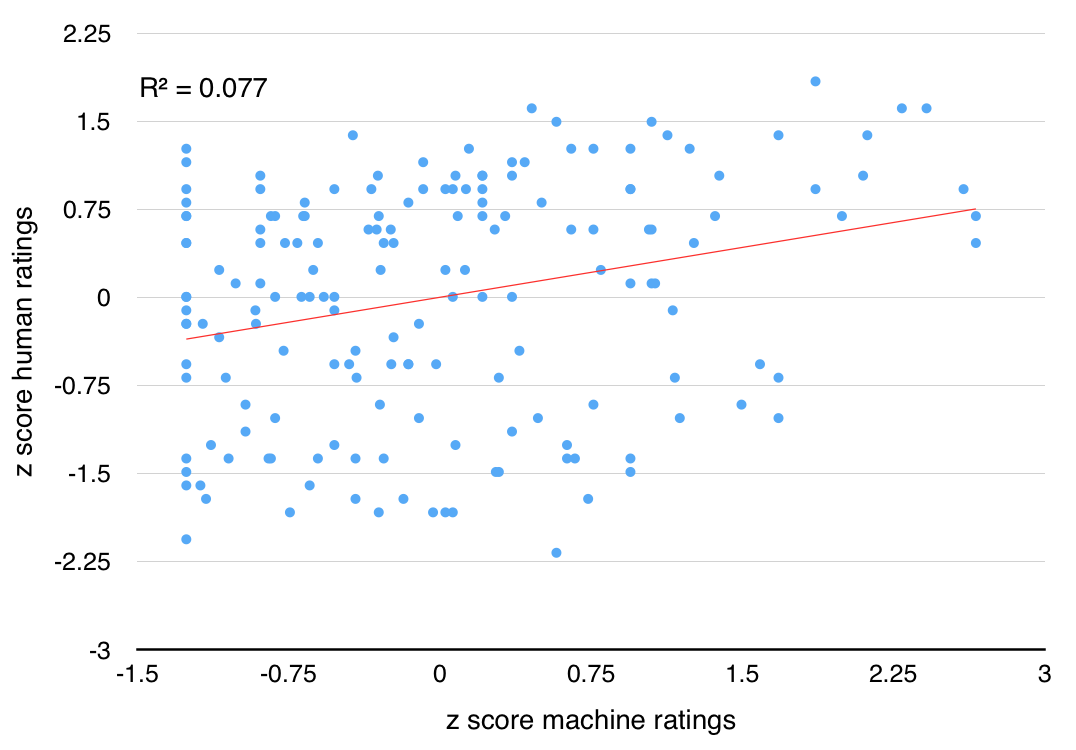
\includegraphics[width=0.8\textwidth]{extract_z_scores}
      \end{figure}

      \begin{figure}[h]
        \caption{\textcolor{red}{or the results can be presented like this. group the human scores 1-5, then for each score plot the corresponding machine score in the box plot}}
        \centering
        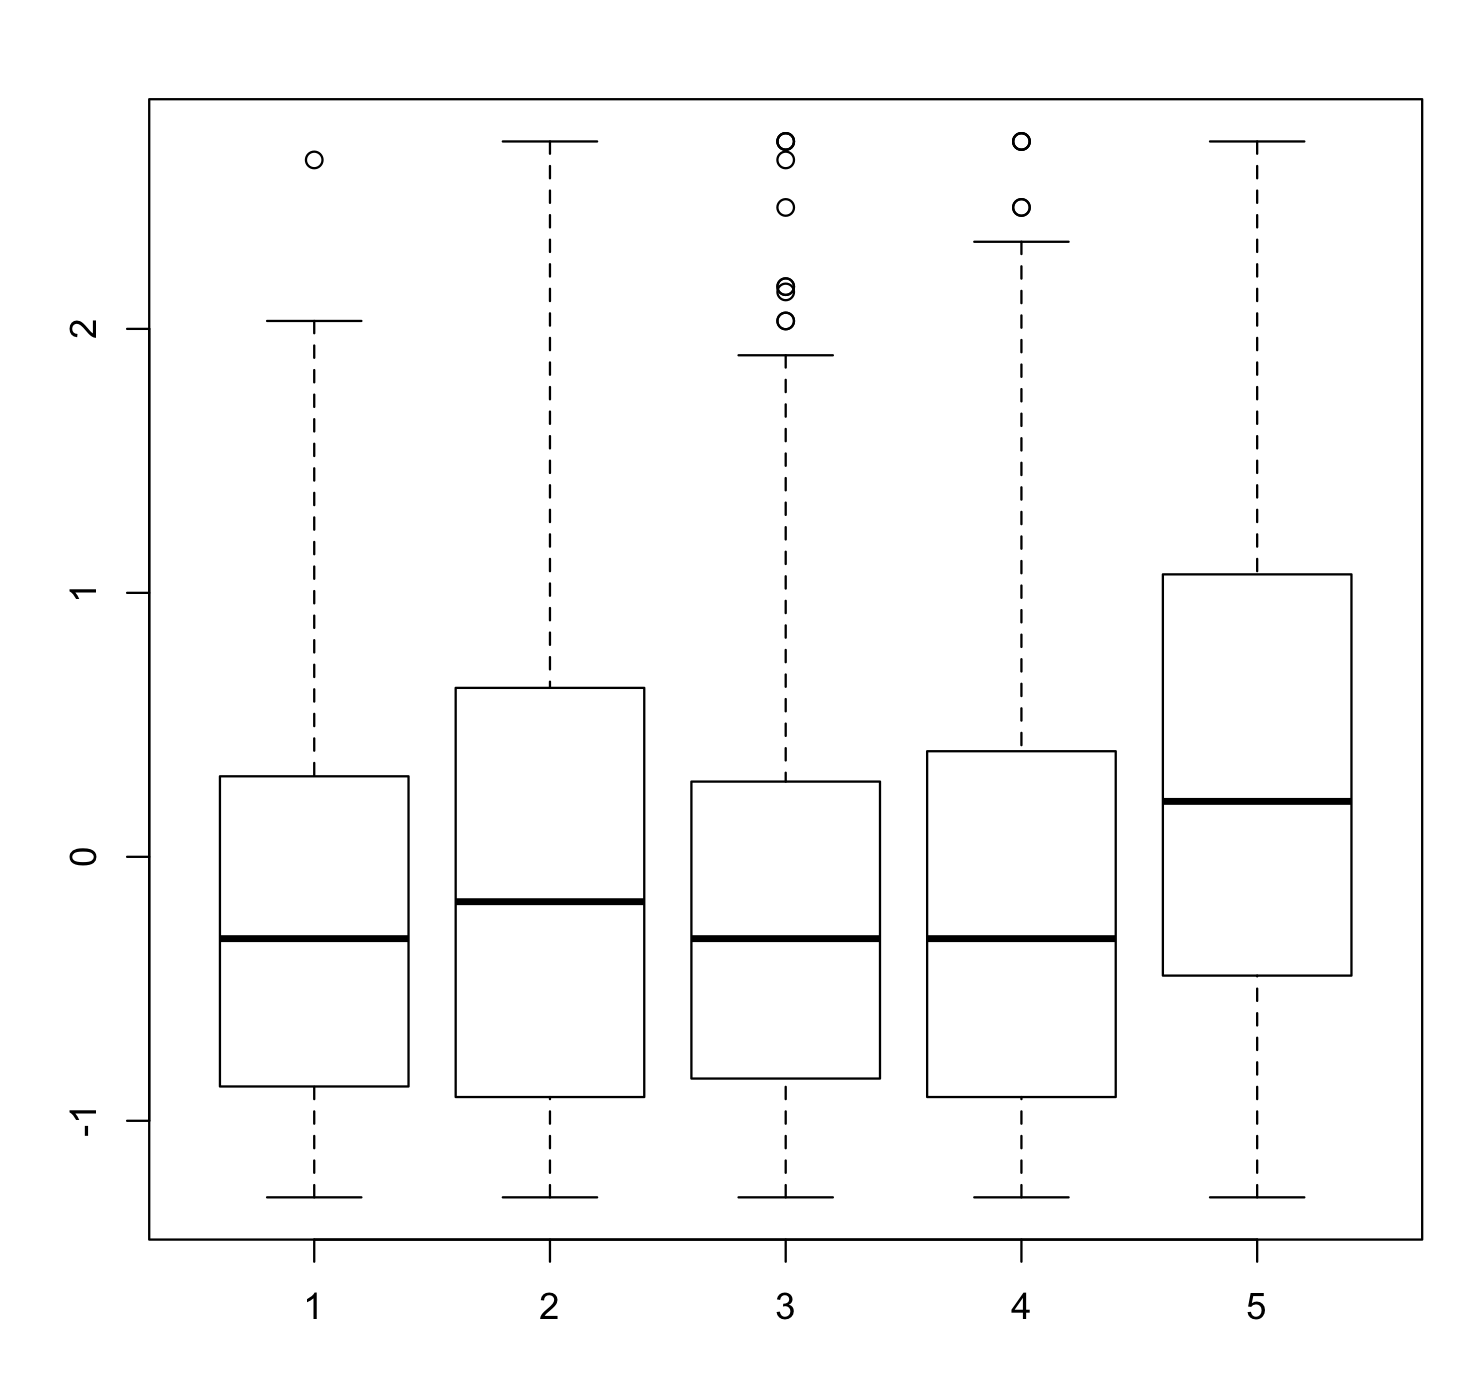
\includegraphics[width=0.8\textwidth]{boxplots}
      \end{figure}

      One selected extract \blockquote{As they pay income taxes} scored particularly poorly with a score of mean score of 2.2/5. However, generally ratings correlate with the extract quality. These results are based on 1587 responses across 18 different clusters of extracts from six topics. The target population of this sample is all clusters of extracts selected for display in summaries.

      Regarding the results of the bigram vs. random summary comparison, there appeared was a preference for the bigram summary. 43\% of participants preferred the bigram summary, 20\% scored them the same and 34\% preferred the randomly generated summaries. Breaking this down by topic, the abortion bigram summary scored more than 5 times the random summary; for creation and healthcare both summaries scored equally. Interestingly, the random god summary scored higher than the accompanying bigram one.

      To test these results against \textbf{H3} we again used a one-sided Sign test. Excluding neutral ratings, the bigram model was successful 24/44 times. Based on this result we are unable to reject \textbf{H3}.

    \tocless\subsection{\textcolor{red}{TBD: Study 3: Section Comparison}}

  \section{Discussion}
    From our results it is clear that both plain \& layout, point-extract based summaries were significantly preferred overall. However, it is not possible to state with any certainty that formatted are preferred over layout summaries. We are also unable to conclude that the bigram model for extract selection is better than random selection.

    \tocless\subsection{Plain vs. Stock}
      In the first study, plain summaries were significantly preferred over stock summaries. Participants comments made reference the comparison factors and comments align with scores allocated. Comparisons that were not captured by the factor ratings were also interesting. Multiple comments made reference to the following comparisons: plain summaries have fewer questions, less surplus information and more content. Comments also made reference to plain summaries being well written with \blockquote{proper English} and \blockquote{complete sentences}. This is particularly interesting when considering the point extraction process.

      There were also five comments that suggest the participant believed the summaries had been written by a human. For example: \blockquote{As I read [STOCK] I felt that I knew the opinion of the writer. With [PLAIN] I could not tell.} and \blockquote{\dots clearer where the author is coming from}. References were also made to higher level properties of the summaries such as \blockquote{logical flow}, \blockquote{relies on fallacy}, \blockquote{explains the reasoning} as well as factual correctness.

      In summary, based on their comments, participants acknowledge succinctness, variety and informativeness even without the explanations and structure of the layout summaries.

    \tocless\subsection{Layout vs. Stock}
      Similarly, layout summaries were significantly preferred over stock summaries. References to organisation doubled in the comments justifying scores allocating scores for this comparison. Readability and the idea of assimilating information was also a common factor cited in justifications for choosing layout summaries. Interestingly there was also an increase in the number of references to `points'.

      Only one comment made a direct reference to `categories' (sections) of the summary. There was one comment that suggested the related points where distracting. We expected there to be more references to summary sections. There were fewer comments that suggested the participants believed the summaries to be written by a human when comparing layout and stock. This is perhaps because the sections hint at a more structured and mechanized approach.

    \tocless\subsection{Layout vs. Formatted}
      This comparison was more divisive. Based on our results we cannot state, for our comparison factors, that the formatted summary style is significantly better. The highlighting of topics and keywords gets varied comments. Those who like the formatting suggest it is easier to read quickly while those that disliked it claim it was distracting and unnecessary. Positive comments such as \blockquote{Highlighting important words makes the text easier to follow; more aesthetically pleasing; and simpler to read.} and \blockquote{Having keywords highlighted allows me to be able to quickly identify and distinguish between the aspects of the topic.} suggest that the participants were able to make use of the formatting. However, comments like: \blockquote{The keywords are bold too often and become a distraction to the reader.} and \blockquote{I don't think it is necessary to make the keywords and topic words bold.} give reasons to remove the additional formatting.

      Interestingly, there were also multiple comments that suggested participants did not notice that \textit{only} formatting changed, despite this being communicated in the task instructions. Also of note is the multiple times participants state that their comment is their opinion, this is not common in comments of other comparisons.

      From these results we learnt that reactions to changes in formatting are more varied and more subjective.

    \tocless\subsection{Bigram vs. Random}
      There were references to the two making the same points/reasoning/arguments. This is interesting as it means participants noticed the same points being made under different extracts. Participants that preferred the bigram summary suggested that it was more concise while the random summary contained too much information. Longer extracts, often providing additional information, are made less likely by the length weighting in the bigram model. Participants that preferred the random summary cited that explanations were more complete and that the bigram summary was too basic.

      As with previous comparisons, some comments gave the suggestion that the participants sometimes believed the summary to be written by a human. For example, \blockquote{Side [RANDOM] uses the scientific method and doesn't involve a fake deity at all in the science section.} and \blockquote{[BIGRAM] is definitely college level.}. Such comments suggest that expectation for summary quality is quite high.

      In summary, the results and comments from this comparison appear to suggest that the detail in longer points is valuable if the point is well formed. This makes a case for reducing the effect of the length weighting and including a readability factor when selecting extracts.

    \tocless\subsection{Extract Comparison}
      TBC, when the stats tests are finalized
    \tocless\subsection{\textcolor{red}{TBD: summary sections}}
      TBD: when we have run this experiment
